\chapter{Алгоритм построения маршрутов}

\section{Модели данных}
В этом разделе будут описаны 3 способа представления данных о транспортной системе в виде графа, на котором впоследствии будут применятся алгоритмы для построения маршрутов и доступ к которому будет иметь построитель маршрутов.
\subsection{Статичный граф}
В статичном случае каждое ребро взвешенно функцией $c:E \rightarrow R$, и не имеет параллельных ребер. Для каждого ребра $e=(u, v)$ будем писать иногда $c(u, v)$ вместо $c(e)$. Будем называть такой граф простым взвешенным. Вес ребра можно интерпретировать как среднее время движения, требуемое на преодоление сегмента дороги, или как физическую длину. Длина пути $P$ в таком случае равна $c(P)=\sum_{i=1}^{k}c(e_i)$. Путь $P^*$ будет является кратчайшим в том случае, если не существует другого пути $P'$ с такой же стартовой и конечной вершинами, что и у пути $P^*$, такого, что $c(P')<c(P^*)$.

Можно построить граф транспортных рейсов, который будет соответствовать данному случаю. Для этого возьмем на вершину графа транспортный узел, а движение транспорта от одного транспортного узла до другого -- за ребро. За вес ребра будет принята длина сегмента пути, так как она не меняется с течением времени. Далее на таком графе можно применить алгоритм Йена и найти $k$ путей.

К сожалению, такой подход имеет ряд существенных минусов. Во-первых, будет доступна только одна естественная сортировка -- по количеству пересадок, так как в данном случае это будет просто количество ребер. Во-вторых, поддержка временных интервалов потребует дополнительных вызовов алгоритма для того, чтобы гарантированно получить те маршруты, которых попадают в определенные временные границы. В-третьих, это размер графа, который зависит от количества остановок каждого транспорта за период даты продаж.

\begin{figure}[!h]
	\centering
	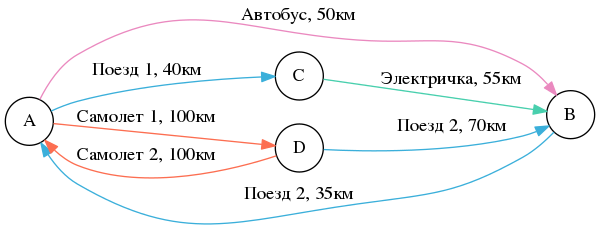
\includegraphics[width=\textwidth]{static_graph_example.png}
	\caption{Статичный граф с 4 городами и 6 транспортами}\label{fig3}
\end{figure}
\FloatBarrier

\subsection{Граф расписаний}
Традиционно расписания представляются множеством поездов (автобусов, самолетов и т.д.). Каждый поезд посещает последовательность станций (автобусных остановок, аэропортов и т.д.). Для каждой станции, за исключением последней, расписание включает в себя время отбытия, и для каждой станции, за исключением первой, включает в себя время прибытия, как показано в таблице:

Для того, чтобы была возможность математически определить связи, состоящие из нескольких поездов, мы разделим их в элементарные связи. Более формально, мы имеет множество станций $B$, множество остановок $Z_S$ на каждой станции $S \in B$ и множество элементарных связей $C$, чьи элементы $c$ являются кортежами вида $c=\{Z_d,Z_a,S_d,S_a,\tau_d,\tau_d\}$. Такой кортеж интерпретируется как поезд, который отправляется со станции $S_d$ со временем отбытия $\tau_d$ после остановки $Z_d$ и затем следующую остановку $Z_a$ на станции $S_a$ с временем прибытия $\tau_a$. Если $x$ обозначает поле кортежа, то $x(c)$ является значением $x$ в элементарном связи $c$. Событие остановки похожа на идентификатор поезда, но на самом деле является более сложным. Определим событие остановки как последовательное прибытие и отбытие поезда со станции, не осуществляя пересадку. Для соответствующего прибытия элементарной связи $c_1$ и отбывающей связи $c_2$ выполняется $Z_a(c_1)=Z_d(c_2)$. Более того, событие остановки является локальным по отношению к каждой станции. Введем дополнительные события остановки для начала транспортного рейса и для его конца.

\begin{definition}
	Длительность элементарной связи $c$ определяется как $d(c)=\tau_a(c)-\tau_d(c)$.
\end{definition}

На станции или любом другом транспортном узле $S \in B$ возможно совершить пересадку с одного поезда на другой, если время между прибытием и отбытием на станции $S$ больше и равно минимальному времени пересадку -- $minTransferTime(S)$. Аналогично вводится максимальное время -- $maxTransferTime(S)$. Для простоты дальнейших рассуждений примем $minTransferTime = const$ и $maxTransferTime = const$.

Пусть $P=(c_1, ..., c_k)$ будет последовательностью элементарных связей. Определим $dep_i(P)=\tau_d(c_i)$, $arr_i(P)=\tau_a(c_i)$, $S_d(P)=S_d(c_1)$, $S_a(P)=S_a(c_k)$, $Z_d(P)=Z_d(c_1)$, $Z_a(P)=Z_a(c_k)$, $dep(P)=dep_1(P)$, $arr(P)=arr_k(P)$ и $d(P)=arr(P)-dep(P)$. Таким образом, последовательность $P$ будет называться согласованной связью между станциями $S_d(P)$ и $S_a(P)$, для которой выполняются следующие условия:
\begin{enumerate}
	\item Станция отправления $c_{i+1}$ является станцией прибытия $c_i$.
	\item Для минимального времени пересадки соблюдается либо $Z_d(c_{i+1})=Z_a(c_i)$, либо $dep_{i+1}(P)-arr_i(P) \geqslant minTransferTime(S_a(c_i))$ 
\end{enumerate}

Для того, чтобы построить из расписания граф, потребуется получить все маршруты поездов. Граф будет иметь 3 вида вершин, каждая из которых будет содержать время и принадлежать станции. Для каждого элементарной связи $c_1=(Z_1, Z_2, S_1, S_2, \tau_1, \tau_2)$ из станции $S_1$ в станцию $S_2$ на одинаковом поезде мы добавим вершину отправления $S_1d@\tau_1$ на станции $S_1$ со временем отправления $\tau_1$, вершину прибытия $S_2a@\tau_2$ на станции $S_2$ со временем прибытия $\tau_2$ и ребро $S_1d@\tau_1 \rightarrow S_2a@\tau_2$, обозначающее поезду на транспортном средстве со станции $S_1$ на $S_2$. Если транспортное средство продолжает движение со станции $S_2$ во время $\tau_3$, то добавим ребро $S_2a@\tau_2 \rightarrow S_2d@\tau_3$, представляющее собой ожидание транспорта на станции $S_2$. Это возможно, независимо от того, насколько мала разница $\tau_3-\tau_2$.

Для каждой вершины отправления $S_2d@\tau$ добавим вершину пересадки $S_2t@\tau$ с тем же временем и добавим ребро $S_2t@\tau \rightarrow S_2d@\tau$ между ними. Также мы добавим ребро $S_2t@\tau \rightarrow S_2t@\tau'$, идущее ко следующей вершине пересадки по возрастаю времени. Такие ребра будет назвать ребрами ожидания (или ребрами пересадки). Теперь для того, чтобы позволить совершить пересадку после прибытия в вершину $S_2a@\tau_2$, добавим ребро к первой вершине пересадки, для которой выполняется $\tau \geqslant \tau_2 + minTransferTime(S_2)$ и $\tau \leqslant \tau_2 + maxTransferTime(S_2)$. Это даст возможность, совершить пересадку на любой транспортный рейс.
 
\begin{figure}[!h]
	\centering
	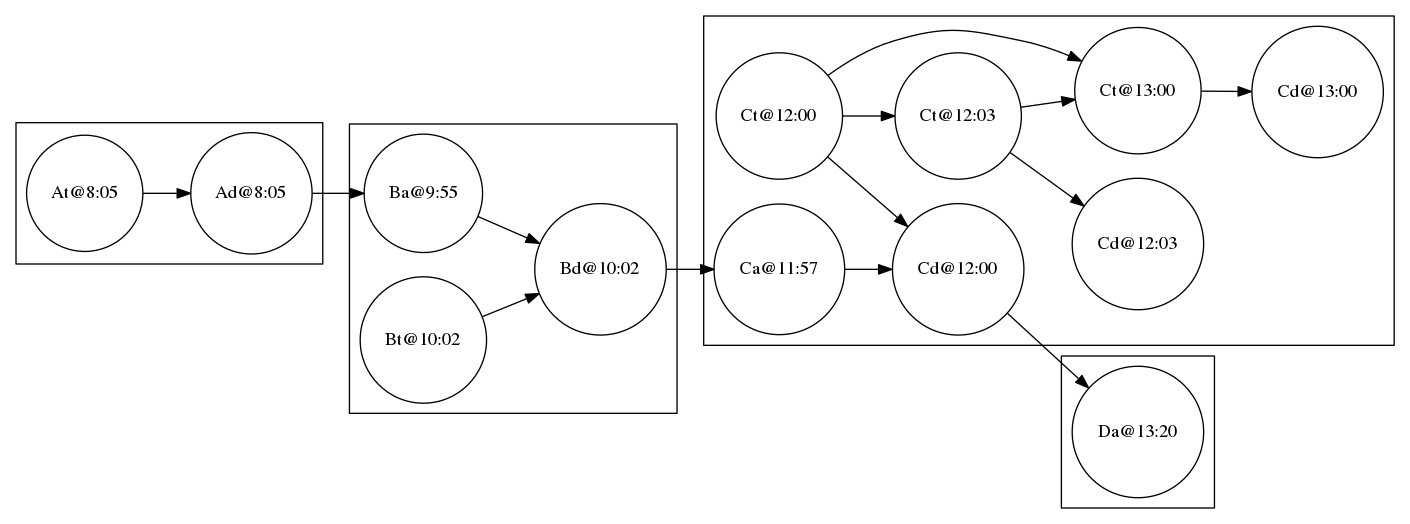
\includegraphics[width=\textwidth]{timetable_graph.png}
	\caption{Для каждого события остановки есть соответствующая вершина. Вес ребра неявно задан по определению длительности элементарной связи. В данном примере $minTransferTime(C)$ равен 10 минутам.}\label{fig4}
\end{figure}
\FloatBarrier 
 
\subsection{Граф рейсов}
Попробуем упростить и в то же время улучшить модель на основе графа расписаний. Заметим, что вершины пересадки $St$ можно удалить из графа без потери информации. Для этого заменим все ребра вида $St@\tau \rightarrow St@\tau'$ на ребра $Sd@\tau \rightarrow Sd@\tau'$. Это возможно сделать, потому что для каждой вершины пересадки $St@\tau$ существует парная ей вершина отправления $Sd@\tau$ с одинаковым временем $\tau$. Также поменяем конец ребер вида $Sa@\tau \rightarrow St@\tau'$ на вершины отправления. Таким образом, поддерживать упорядоченный порядок по времени отправления нужно в самих вершинах отправления.

\begin{figure}[!h]
	\centering
	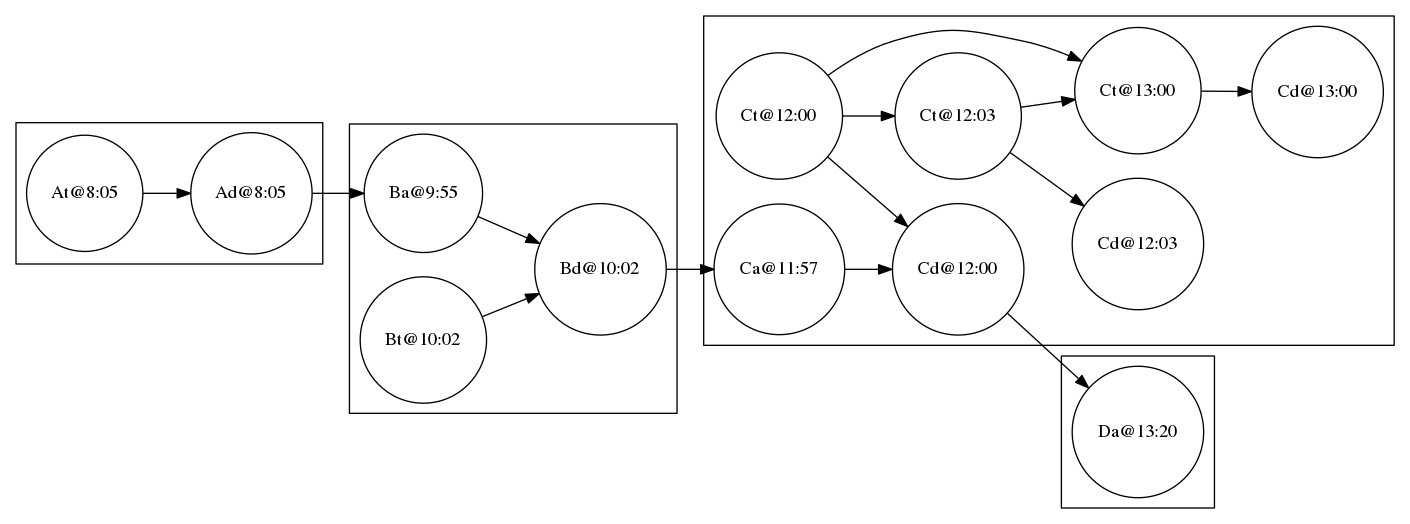
\includegraphics[width=\textwidth]{timetable_graph.png}
	\caption{Для каждого события остановки есть соответствующая вершина. Вес ребра неявно задан по определению длительности элементарной связи. В данном примере $minTransferTime(C)$ равен 10 минутам.}\label{fig4}
\end{figure}
\FloatBarrier 

Следующим шагом улучшения модели будет проведение операции под названием транзитивное замыкание.

\begin{definition}
	В теории графов транзитивным замыканием графа будет является добавление дополнительных ребер между всеми вершинами, между которыми существует путь.
\end{definition}

Наивный способ транзитивного замыкания предполагает добавление ребер между всеми парами вершин отправления $S_id@\tau_i$ и прибытия $S_ja@\tau_j$. Такие ребра будут называться кратчайшими. В них можно хранить информацию о $K_{max}$ кратчайших маршрутах между парой транспортных узлов $S_i$ и $S_j$, где $K_{max}$ -- максимальное количество маршрутов, которые могут быть запрошены клиентским приложением у построителя маршрутов. 

Для того, чтобы сделать полное замыкание графа, нужно построить кратчайшие маршруты от каждой вершины отправления до каждой вершины прибытия. Для такой задачи существует алгоритм Флойда-Уоршелла, который требуем $O(n^3)$ времени, где $n$ -- количество вершин\footnote{Улучшенная версия алгоритма требует $O(n^2\log n)$ времени.} и $O(n^3K_{max})$ памяти.

В итоге, несмотря на всю простоту модели, к сожалению, такой подход крайне неэффективно расходует память и требует огромное время на фазу предварительного расчета. 

\begin{figure}[!h]
	\centering
	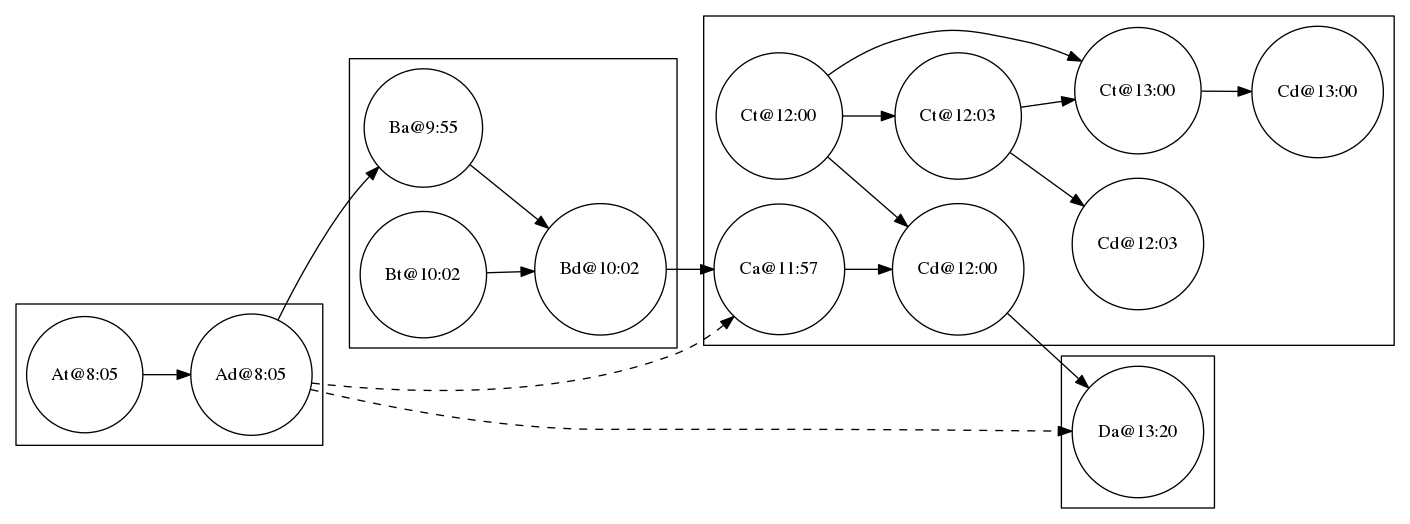
\includegraphics[width=\textwidth]{full_closure_example.png}
	\caption{Для каждого события остановки есть соответствующая вершина. Вес ребра неявно задан по определению длительности элементарной связи. В данном примере $minTransferTime(C)$ равен 10 минутам.}\label{fig4}
\end{figure}
\FloatBarrier 

Улучшенный способ транзитивного замыкания работает локально. Вместо того, чтобы добавлять ребра между всеми парами вершин отправления $S_id@\tau_i$ и прибытия $S_ja@\tau_j$ во всем графе, будем добавлять их только между такими вершинами, построенными на основе конкретного транспортного рейса.

Оценим время и память требуемое для построения такой модели. Пусть $q$ -- количество остановок в одном транспортном рейсе, $n$ -- количество транспортных рейсов. Рассмотрим остановку $Z_i$, где i -- номер остановки в транспортном рейсе. В худшем случае от каждой вершины отправления $S_id@\tau$ будет идти $q-i$ ребер до всех оставшихся вершин прибытия $\forall j > i : S_ja@\tau_j$. Аналогично до каждой вершины $S_ia@\tau$ будет идти $i$ ребер от всех вершин прибытия $\forall j < i : S_ja@\tau_j$. Не сложно заметить, что на один транспортный рейс таким образом будет приходиться $\dfrac{q^2}{2}$ ребер. Требуемое время, которое потребуется для построения модели, равно $O(q^2n)$, не считая времени на получение минимальной вершины, а суммарная память -- $O(q^2n)$ для ребер и $O(qn)$ для вершин.

\begin{algorithm}[!h]
	\caption{Алгоритм построения транзитивного замыкания}\label{lst3}
	\begin{algorithmic}
		\Function{Closure}{$runs$, $stops$}
		\For{$ run \in runs$}
		\For{$i = 0$ to $size(stops[run])$}
		\State $S \gets stops[run][i]$ \Comment{получаем из события остановки станцию}
		\State Создаем вершину $S_ia@\tau_i$
		\For{$j = 0$ to $i - 1$}
		\State создаем ребро $S_jd@\tau_j \rightarrow S_ia@\tau_i$
		\EndFor
		\State Создаем вершину $S_id@\tau_i$
		\For{$j = i + 1$ to $size(stops(run))$}
		\State создаем ребро $S_id@\tau_i \rightarrow S_ja@\tau_j$
		\EndFor
		\State $minNode \gets getMinNode(S_id@\tau_i)$ \Comment{получаем минимальную вершину отправления в порядке сортировки по времени}
		\State Создаем ребро пересадки $S_ia@\tau_i \rightarrow minNode$
		\EndFor
		\EndFor
		\EndFunction
	\end{algorithmic}
\end{algorithm}
\FloatBarrier 

Попробуем изменить подход и использовать единую вершину остановки. Для этого назовем элементарной остановкой кортеж из 4 элементов $St=(i, r, s, \tau)$, хранящий информацию о номере остановки $i$, транспортном рейсе $r$, станции $s$, а также метки времени $\tau$, которая будет хранить либо время отправления, либо прибытия в зависимости от того, как мы будем её интерпретировать. Задачу о хранении возможных пересадок перенесем из модели графа в модели транспортных рейсов, для которых известны также сами события остановок. Создадим по массив в транспортном рейсе размером с количество его остановок, который будет хранить неупорядоченные списки элементарных остановок.

\begin{algorithm}[!h]
	\caption{Алгоритм построения пересадок}\label{lst4}
	\begin{algorithmic}
		\Function{buildTransfers}{$runs$}
		\For{$ r \in runs$}
		\State $transfers[r] := \emptyset$ \Comment{Список пересадок для транспортного рейса $r$}
		\For{$i = 0$ to $|W(r)| - 1$}
			\State $w := W(r)[i]$
			\State $s := S(w)$ \Comment{по точке маршрута можно получить станцию}
			\If{$i \neq 0$} \Comment{игнорируем $i = 0$, так как только сели на поезд и пересадку делать не нужно в любом случае}
				\State $st_a := (i, R, s, \tau_a(w))$ {Текущая элементарная остановка со временем прибытия}
				\State $T_a(s).put(\tau_a(w), st_a)$ {Помещаем остановку в расписание прибытий станции $s$}
				\For {$(\tau, st') \in T_a(s) : \tau - \tau_a(w) \in [T_{min}(s), T_{max}(s)]$}
					\If{$ R(st') \neq r$} \Comment{Исключаем пересадку на текущий транспорт}
						\State $transfers[i].add(st')$
					\EndIf
				\EndFor
			\EndIf
			\If{$i \neq |W(r)| - 1$} \Comment{не делаем пересадки на поезд, который уже находится на своей конечной станции}
				\State $st_d := (i, R, s, \tau_d(w))$
				\State $T_d(s).put(\tau_a(w), st_d)$
				\For {$(\tau, st') \in T_a(s) : \tau - \tau_d(w) \in [-T_{max}(s), -T_{min}(s)]$}
					\If{$ R(st') \neq r$ \textbf{and} $ i \neq 0$} \Comment{игнорируем $i = 0$, так как только сели на поезд и пересадку делать не нужно в любом случае}
						\State $transfers[i].add(st_d)$
					\EndIf
				\EndFor
			\EndIf
		\EndFor
		\EndFor
		\EndFunction
	\end{algorithmic}
\end{algorithm}

Также нам потребуется хранить 2 структуры данных с поддержкой быстрого поиска элементов в определенной границе. Такой структурой данных может быть красно-черное дерево, поддерживающее поиск элемента за $O(\log n)$, или аналогичный по асимптотике и возможностям список с пропусками. Обе эти структуры помогут быстро находить элементарные остановки во множестве событий прибытия $T_a(s)$ и отбытия $T_d(s)$ на станцию $s$.

Рассмотрим, как теперь будет строиться модель. Построение модели можно реализовать инкрементально, то есть добавлять в модель по одному транспортному рейсу. Для каждого такого рейса создается массив $transfers$, который хранит на $i$ позиции список элементарных остановок отправления, на которые можно пересесть с текущего рейса на $i$ точке маршрута. Пустой список означает, что либо в точке маршрута другой транспорт не останавливается, либо он не подходит по критериям пересадки, то есть не соблюдаются допустимые интервалы времени, связанные с $T_{min}$ и $T_{max}$. Для каждого рейса выполняется обход его маршрутных точек с обновляем пересадок в каждой из них.
\FloatBarrier 

\section{Построение маршрутов}
Теперь у нас есть эффективная модель в виде графа рейсов для хранения информации о транспортной сети. На каждой станции поддерживается несколько структур данных для определения прибывающих и отбывающих поездов по конкретному интервалу времени. Также для каждого транспортного рейса можно быстро узнать возможные пересадки на пути всего следования поезда. Попробуем придумать эффективный алгоритм поиска маршрутов на заданной модели.

\subsection{Дополнение временных интервалов}
Типичный запрос к построителю маршрутов выглядит как кортеж из 5 элементов $(s_d, t_d, s_a, t_a, k)$, где $s_d$ и $s_a$ -- станции отправления и прибытия соответственно, $t_d=(\tau_{d1}, \tau_{d2})$ и $t_d=(\tau_{a1}, \tau_{a2})$ -- требуемые интервалы времени, $k$ -- количество маршрутов. Временные интервалы бывают 3 типов:
\begin{enumerate}
	\item Фиксированные
	\item Полубесконечные
	\item Бесконечные
\end{enumerate}

\begin{algorithm}[!h]
	\caption{Приведение интервалов к фиксированному виду}\label{lst5}
	\begin{algorithmic}
		\Function{normalizeTime}{$t_a$, $t_d$}
		\If{$t_{d1} = -\infty$ \textbf{or} $ t_{d1} < T_{now} $}
			\State $t_{d1} := T_{now}$
		\EndIf
		\If{$t_{a2} = \infty$ \textbf{or} $t_{a2} > T_{end}$}
			\State $t_{a2} := T_{end}$
		\EndIf
		\If{$t_{d2} = \infty$ \textbf{or} $t_{d2} > T_{end}$}
			\State $t_{d2} := t_{a2}$
		\EndIf
		\If{$t_{a1} = \infty$ \textbf{or} $t_{a1} < T_{now}$}
			\State $t_{a1} := t_{d1}$
		\EndIf
		\EndFunction
	\end{algorithmic}
\end{algorithm}

Фактически бесконечность в данном случае условная, потому что время построителя маршрутов всегда ограничено снизу текущим временем построителя $T_{now}$, а сверху -- временем конца продаж $T_{end} = T_{now} + T_{len}$, где $T_{len}$~-- интервал продажи билетов. Для упрощения работы с интервалы их имеет смысл привести к фиксированному времени\footnote{Для чего это сделано будет более понятно в следующей главе с конкретной реализацией}.
\FloatBarrier 

\subsection{Фаза инициализации}
Идея алгоритма состоит в следующем: будем генерировать состояния, в которых можем находится на пути следования до точки назначения. В процессе генерации будем осуществлять фильтрацию маловероятных состояний и невозможных с точки зрения требований к маршруту.

В качестве допустимого состояния будет выступать кортеж из двух элементов $e=(st, m)$, где $st$ -- элементарная остановки, $m$ -- количество совершенных пересадок. 

В процессе работы нам потребуется множество вспомогательных структур данных, в которые будут записываться промежуточные результаты. Часть из них будут являться пересадочными массивами. Под этим термином будут подразумеваться массивы, индекс в которых будет указывать на текущее число рассматриваемых пересадок. Например, элемент массива $array[3]$ будет хранить данные для состояний, которые уже совершили 3 пересадки.

\subsubsection{Вспомогательные структуры данных}
Помимо структур данных нам потребуются несколько новых моделей, в которых мы будем хранить совершаемые действия, чтобы прийти в некоторое состояние $e$. Такие модели будем называть сегментами. В общем случае будет существовать 2 вида сегментов:
\begin{enumerate}
	\item Прямой сегмент ($A-B-C$). Он будет определять действия, совершаемые в процессе обхода графа от событий отправления. Он потребуется нам при сортировке по времени отправления;
	\item Обратный сегмент ($B-C-D$). Он будет определять действия, совершаемые в процессе обхода графа от событий прибытия. Он потребуется нам при всех остальных видах сортировок;
\end{enumerate}

Каждый сегмент состоит из 3 элементарных остановок. Остановка $А$ является событием отправления 1 поезда, $B$ -- его прибытие, $C$ -- отправление 2 поезда, $D$ -- прибытие. Можно заметить, что часть $B-C$ совпадает у обоих сегментов. Это часть является неявных событием пересадки, с помощью которого можно однозначно конвертировать сегменты друг в друга, а также находить пересечения. Как будет показано позже, это поможет реализовать двунаправленных обход графа рейсов. 

\begin{figure}[!h]
	\centering
	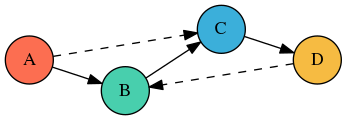
\includegraphics[width=0.75\textwidth]{segments_example.png}
	\caption{Совмещение прямого и обратного сегментов. Пунктирные линии показывают следующее состояние, которое будет добавлено в очередь.}\label{fig4}
\end{figure}

На самом деле любая сортировка может быть выполнена с наличием только одного вида сегментов, потому что путем их обхода можно из одного получить другой.

\begin{itemize}
		\item $expanded$ -- пересадочный массив множеств посещенных состояний;
		\item $explored$ -- пересадочный массив множеств рассмотренных состояний
		\item $queue$ -- очередь состояний;
		\item $pathsCount$ -- пересадочный массив хеш-таблиц для остановок, хранящий число возможных маршрутов;
		\item $successors$ -- пересадочный массив хеш-таблиц для остановок, хранящий список прямых сегментов;
		\item $predecessors$ -- пересадочный массив хеш-таблиц для остановок, хранящий список обратных сегментов;
\end{itemize}

\subsubsection{Заполнение вспомогательные структур}

\begin{algorithm}[!h]
	\caption{Заполнение вспомогательных структур}\label{lst5}
	\begin{algorithmic}
		\For {$s \in sources$}
			\State $departures.add(P(s))$ \Comment{Добавляем транспортный узел в список узлов отправления}
			\State $pathsCount[0].put(s, 1)$ \Comment{Из остановки можно доехать в саму себя за 0 пересадок только 1 способом}
			\State $st = (s, 0)$ \Comment{Создаем состояние с событием отправления $s$ и $0$ совершенных пересадок}
			\State $explored.add(st)$ \Comment{Добавляем состояние в список рассмотренных}
			\State $queue.add(st)$ \Comment{Добавляем в очередь на обработку}
		\EndFor
		\For {$t \in targets$}
			\State $arrivals.add(P(t))$ \Comment{Добавляем транспортный узел в список узлов прибытия}
		\EndFor
	\end{algorithmic}
\end{algorithm}

\FloatBarrier
\subsection{Фаза обхода}

\[
predessors[j][v]=\{(u, i) : \exists \langle (u, i), (v, j) \rangle\}
\]

\section{Сортировка маршрутов}

\subsection{Количество пересадок}
\begin{algorithm}[!h]
	\caption{Заполнение переданного уровня}\label{lst5}
	\begin{algorithmic}
		\Function{fillLevel}{$level$, $k$}
		\For{$t \in targets$}
			\State $incomming := predecessors[k][t]$;
			\For {$s \in incoming$}
				\State $level.add(k, s)$
			\EndFor
		\EndFor
		\EndFunction
	\end{algorithmic}
\end{algorithm}

\begin{algorithm}[!h]
	\caption{Подготовка сортировки по количеству пересадок}\label{lst5}
	\begin{algorithmic}
		\Function{sortedByTransfersCount}{$level$, $k$}
		\State $unvisited := \emptyset$ \Comment{случайный уровень}
		\If {$direction = ASC$}
			\For {$i = 0$ \textbf{to} $maxTransfersCount$}
				\State \Call{fillLevel}{unvisited, i}
			\EndFor
		\Else
		\For {$i = maxTransfersCount$ \textbf{downto} $0$}
			\State \Call{fillLevel}{unvisited, i}
		\EndFor
		\EndIf
		\State \Return $unvisited$
		\EndFunction
	\end{algorithmic}
\end{algorithm}

\begin{algorithm}[!h]
	\caption{Заполнение переданного уровня}\label{lst5}
	\begin{algorithmic}
		\Function{fillLevel}{$level$, $k$}
		\For{$t \in targets$}
		\State $incomming := predecessors[k][t]$;
		\For {$s \in incoming$}
		\State $level.add(k, s)$
		\EndFor
		\EndFor
		\EndFunction
	\end{algorithmic}
\end{algorithm}

\FloatBarrier
\subsection{Время прибытия}

\subsection{Время отправления}
\begin{algorithm}[!h]
	\caption{Строим и возвращаем следующий маршрут по множеству исходящих сегментов}\label{lst5}
	\begin{algorithmic}
		\Function{forwardNext}{$level$, $k$}
		\While {$stack \neq \emptyset$}
			\State $level := stack.peek()$ \Comment{получаем текущий уровень в стеке}
			\If {$level \neq \emptyset$}
				\State $st = level.poll()$ \Comment{извлекаем состояние из уровня}
				
				\State $b := st.segment.B()$
				\State $t := st.transfers$
				
				\If {$arrivals\text{ содержит }P(b)$} \Comment{Маршрут найден, так как пришли в точку отправления}
				\State $path = \Call{buildFrom}{state, true}$ \Comment{Строим маршрут}
				\State $candidates.add(path)$ \Comment{Добавляем маршрут в список кандидатов}
				\If {$|path| > 1$}
				\State $stack.poll()$
				\EndIf
				\EndIf
				
				\State $outgoing := successors[t][b]$;
				\If {$outgoing \neq \emptyset$}
				\State $level' := \emptyset$ \Comment{создаем новый случайный уровень}
				\For {$segment \in outgoing$}
				\If {$segment\text{ является пересадкой}$}
				\State $t' = t + 1$
				\Else
				\State $t' = t$
				\EndIf
				\State $st' := (st, segment, t')$
				\State $level'.add(st')$
				\EndFor
				\State $stack.push(level')$
				\EndIf
			\Else
				\State $stack.poll()$ \Comment{на текущем уровне не осталось состояний, можно подняться выше}
			\EndIf
		\EndWhile
		\EndFunction
	\end{algorithmic}
\end{algorithm}

\FloatBarrier
\subsection{Время в пути}

\section{Построение фильтров}
Построение фильтров также, как и поиск маршрутов, состоит из двух фаз: предварительного расчета и основной. В первом случае модели данных, которые отвечают за транспортные средства переводятся в удобные и компактные модели, которые будут использоваться при непосредственном поиске маршрутов. Во втором случае готовые структуры данных будут позволять на этапе фазы обхода графа рейсов собирать композитные фильтры для каждой остановки с помощью динамического программирования. Также как и случае подсчета количества маршрутов мы построим динамику, которая будет позволять определять доступные параметры фильтрации для пары элементарных остановок.

\subsection{Косвенные признаки}
В фазе предварительного расчета мы будем извлекать косвенные признаки из моделей транспортных средств. Как было описано в главе 1, такими признаками может быть тип транспорта, номер поезда или тип места в самолете и т.д. Для удобной работы с ними мы разделим все признаки по функциональным типам, то есть, например, признак "перевозчик" у поезда и самолета будут отнесены к разных типам признаков. Это позволит нам логически отделять на этапе отдачи результата клиентскому приложению.

В качестве компактной модели свойств $Pr=\{(t,\{(v, c)\})\}$, хранящей признаки, будет выбрана хеш-таблица из типа признака $t$ в хеш-таблицу значений признака $v$ в количество свободных мест $c$, которые удовлетворяют ему. Например, есть 1 поезд с 3 вагонами (один вагон имеет 20 мест): 2 из них купе, 1 - плацкарт. Из них в плацкарте половина верхних мест, а другая половина - нижних. Тогда будет создан объект свойств для поезда со следующими записями:
\begin{itemize}
	\item Тип транспорта
	\begin{itemize}
		\item (Поезд, 60)
	\end{itemize}
	\item Тип вагона
	\begin{itemize}
		\item (Купе, 40)
		\item (Плацкарт, 20)
	\end{itemize}
	\item Тип места
	\begin{itemize}
		\item (Верхнее, 20)
		\item (Нижнее, 20)
	\end{itemize}
\end{itemize}

Как можно заметить на данном примере, свойства не хранятся в виде иерархии функциональных зависимостей. Это сделано для экономного расхода памяти, а также для упрощения операций со свойствами в процессе выполнения динамики по свойствами. Функциональные зависимости известны заранее и задаются вручную в специальном объекте, о котором речь пойдет позже.

Теперь нужно ввести 2 операции в пространстве свойств признаков, которые будут называться минимум и максимум. Обе операции будут являться ассоциативными, то есть:
\[
(x\circ y)\circ z=x\circ(y\circ z)\text{ для любых элементов }x,\;y,\;z.
\]

Минимум на свойствах работает как минимум количества свободных мест по всем парам признаков $\langle t, v \rangle$. При этом работает правило дополнения, то есть если пара присутствует в свойстве $A$, но отсутствует в $B$, то берется число свободных мест из $A$.

\begin{algorithm}[!h]
	\caption{Минимум из пары свойств}\label{lst5}
	\begin{algorithmic}
		\Function{min}{$Pr_a$, $Pr_b$}
		\If{$Pr_a = \emptyset$}
			\State \Return $Pr_b$
		\EndIf
		\If{$Pr_b = \emptyset$}
		\State \Return $Pr_a$
		\EndIf
		\State $Pr_r := \emptyset$ \Comment{Результирующее свойство}
		\For{$ \langle t, v\rangle : Pr_a \cup Pr_b$}
			\State $Pr_r[t][v] = min(Pr_a[t][v], Pr_b[t][v])$
		\EndFor
		\For{$ \langle t, v\rangle : Pr_a \setminus Pr_b$}
			\State $Pr_r[t][v] = Pr_a[t][v]$
		\EndFor
		\For{$ \langle t, v\rangle : Pr_b \setminus Pr_a$}
			\State $Pr_r[t][v] = Pr_b[t][v]$
		\EndFor
		\State \Return $Pr_r$
		\EndFunction
	\end{algorithmic}
\end{algorithm}

Максимум на свойствах работает аналогично минимуму, только для количества свободных мест операция меняется на максимум.

\subsection{Осуществление фильтрации}
В фазе обхода при построении маршрутов для каждой элементарной остановки генерировались все возможные сегменты, которые являлись пересадочными и конечными. Таким образом, чтобы избежать попадание в следующую элементарную остановку, нужно фильтровать соответствующий сегмент, поэтому в процессе генерации каждому сегменту должно сопоставляться свойство, хранящее признаки для транспортного средства, отправляющегося из остановки $A$\footnote{Для упрощения рассматривается прямой сегмент, для обратного будет остановка прибытия $D$.}

В итоге, мы должны хранить свойства для каждого отрезка пути, соединяющего смежные маршрутные точки. Так как сегмент является множеством последовательно соединенных отрезков пути следования, то свойство сегмента является минимумом из всех свойств отрезков, входящих в него:
\[
Pr_s=\min_{i \in s}{Pr_i}
\]

Для того, чтобы ускорить построение свойства сегмента можно воспользоваться деревом отрезков, позволяющее находить результат операции на интервале за $O(\log q)$ времени и требующее $O(2q)$ памяти, где $q$ -- число маршрутных точек транспортного рейса. В качестве операции будет взята операция минимума свойств. Это возможно, так как определенный ранее минимум ассоциативен, так же имеет нейтральный элемент -- пустое свойство (пустую хеш-таблицу). Таким образом, множество свойств являются моноидом, который можно применять в дереве интервалов.

\subsection{Функциональные зависимости}

\subsection{"Белые" и "черные" фильтры}

\chapterconclusion